\section{Durchführung}
\label{sec:Durchführung}

Ein Bild des Versuches befindet sich in \autoref{fig:1}.
\begin{figure}[H]
    \centering
        \centering
        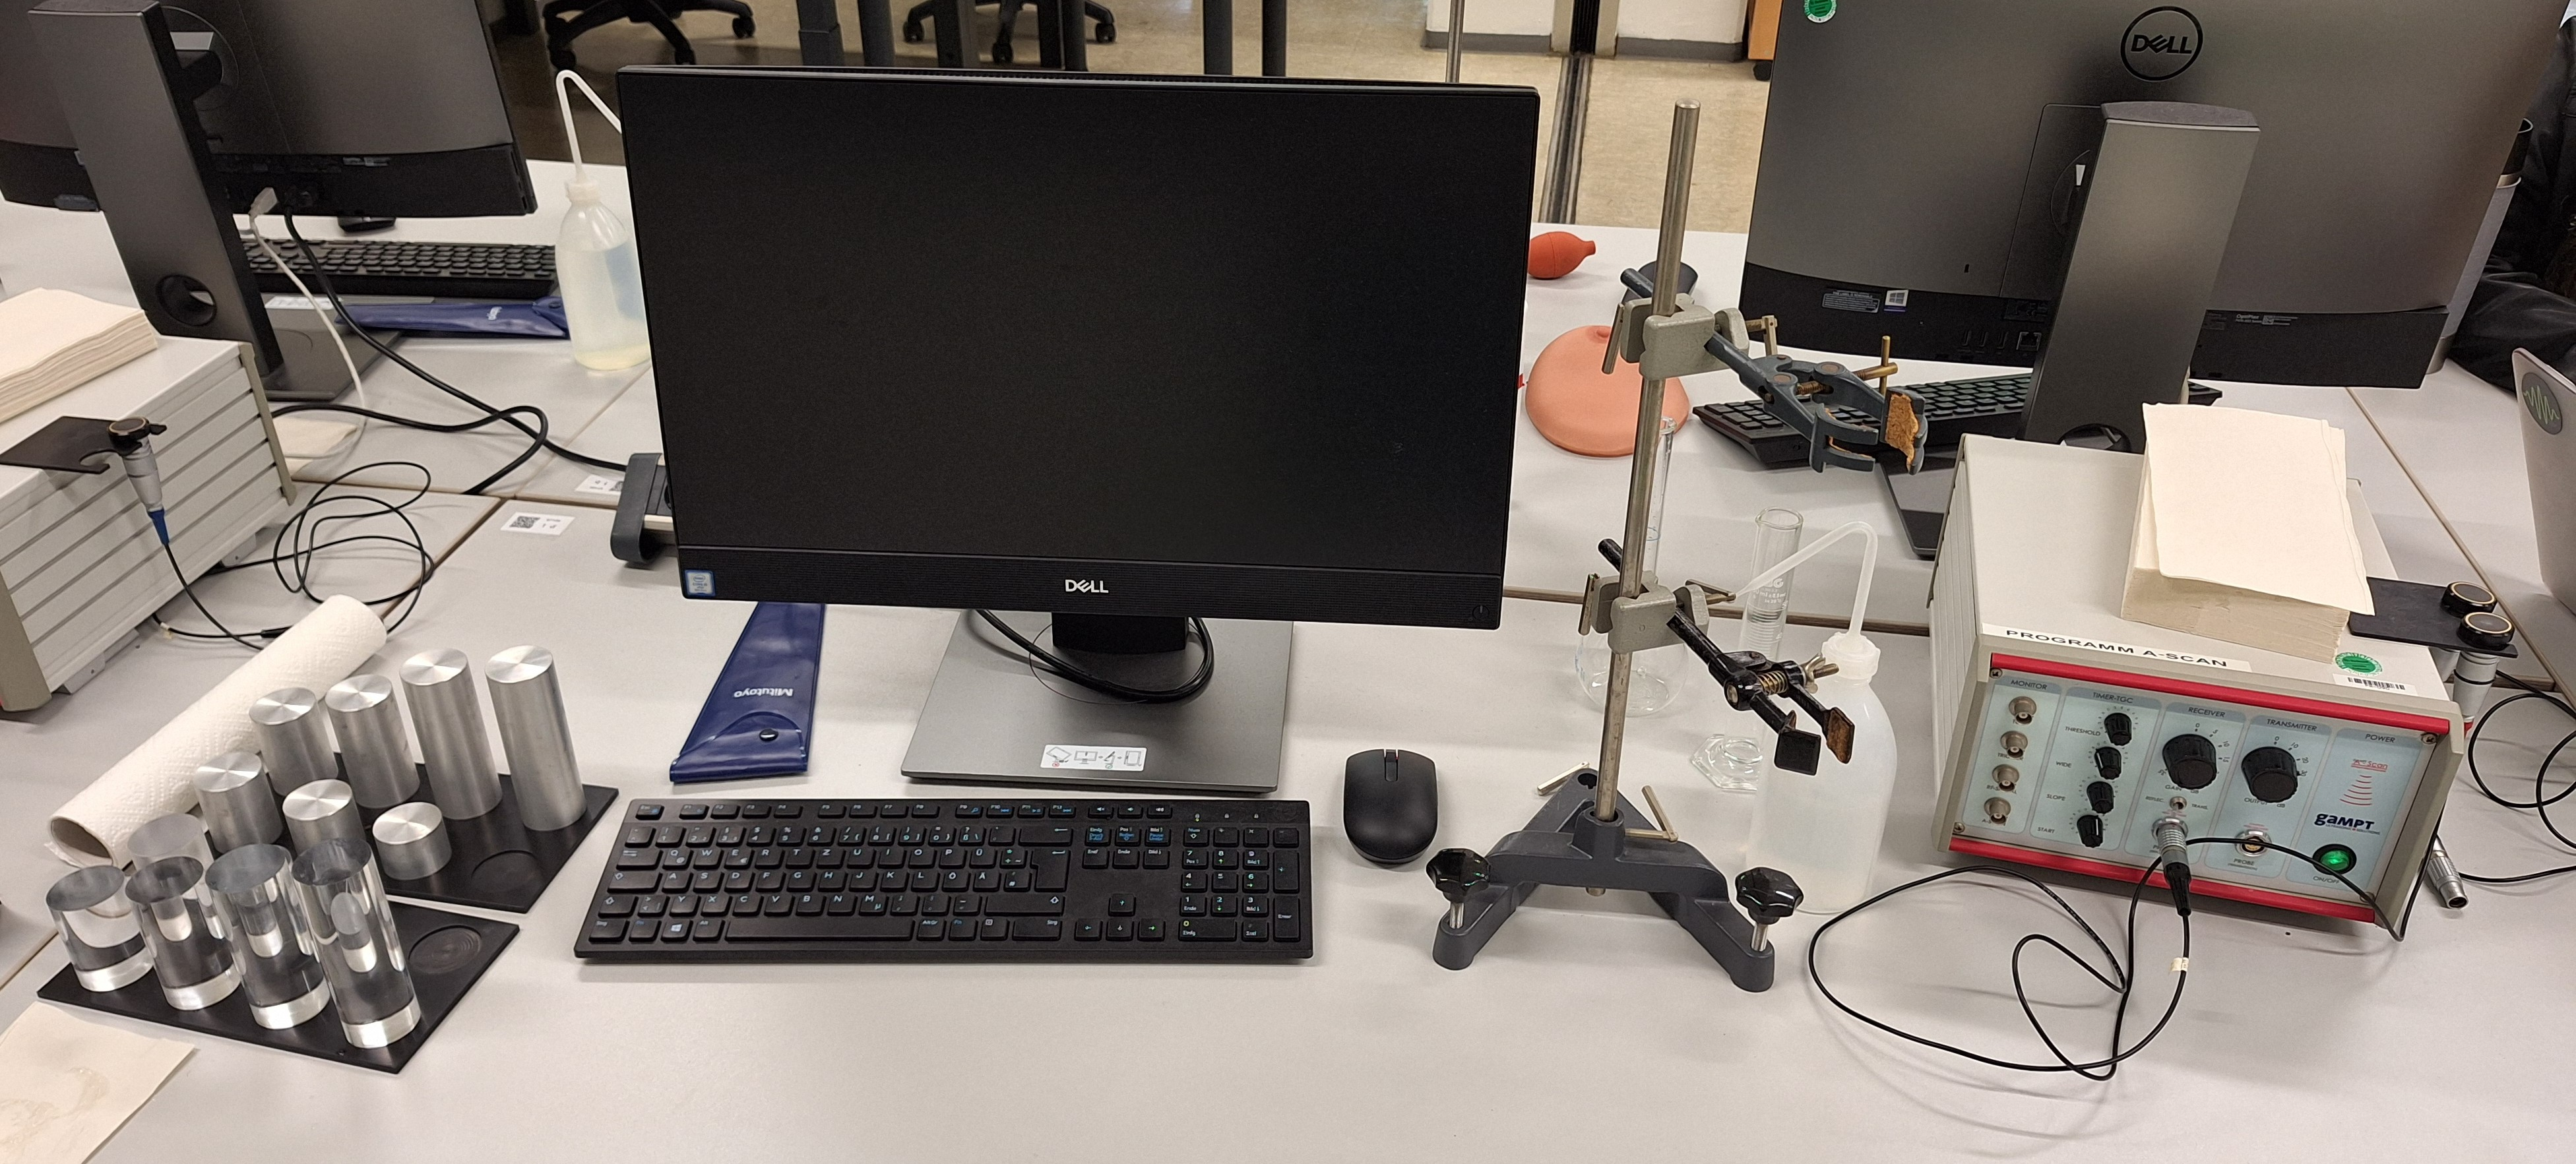
\includegraphics[width=\textwidth]{bilder/versuch.jpg}
        \caption{Darstellung des Experiments.}
    \hfill
    \label{fig:1}
\end{figure}
\noindent Zu sehen sind einerseits die zu untersuchenden Zylinder links, andererseits 
der Computer zum Detektieren der Daten in der Mitte und der Ultraschallgenerator 
ganz rechts. Dieser ist kompatibel mit verschiedenen Ultraschallsonden, in diesem 
Versuch werden diese mit einer Frequenz von $f = 1 \unit{\mega\hertz}$ und 
$f = 2 \unit{\mega\hertz}$ betrieben. Der Computer ist mit dem Programm $A-Scan$ 
ausgestattet, welches Amplituden und Laufzeiten verarbeitet.

\subsection{Programm und Geräteeinstellungen}
Zuerst wird ein Acrylzylinder (in diesem Fall der zweit-kleinste) unter Verwendung 
von destilliertem Wasser unter die $2 \unit{\mega\hertz}$-Sonde gekoppelt. 
Dann wird der A-Scan gestartet. Das Signal wird so weit verstärkt, dass 4 
Amplituden zu erkennen sind. Sie entstehen durch Reflexionen im Inneren des 
Zylinders. Für 5 Schwingungen werden die Perioden gemessen.

\subsection{Bestimmung der Schallgeschwindigkeit in Acryl und Aluminium}
Für die Schallgeschwindigkeitsbestimmung werden die Zylinder zunächst mit einer 
Schieblehre abgemessen. Anschließend werden die Laufzeiten durch alle Zylinder 
mittels A-Scan ermittelt (ebenfalls mit der $2 \unit{\mega\hertz}$-Sonde). 
Ebenso werden jeweils auch zwei gekoppelte Zylinder zur Untersuchung hinzugezogen
(in diesem Fall der 2.- und 3. kleinste).

\subsection{Bestimmung der Dämpfung}
Wie bei der Bestimmung der Schallgeschwindigkeit wird der Versuch an 8
unterschiedlichen Zylinderhöhen durchgeführt, jedoch nur von einem Material, 
in diesem Fall: Aluminium. Genutzt werden beide Sonden.

\subsection{Kalibrierkurve}
Für die Bestimmung der Kalibrierkurve werden die $2 \unit{\mega\hertz}$-Sonde, 
ein Erlenmeyer-Kolben und eine Halterung für beide Komponenten sowie Ultraschallgel 
verwendet. Der Kolben wird mit $50 \unit{\milli\liter}$ aufgefüllt und eingehängt,
direkt darunter wird unter Verwendung des Gels die Sonde gekoppelt. Daraufhin 
kann die Messung beginnen: Es werden die Laufzeiten in Abhängigkeit der Füllmenge 
ermittelt, diese wird immer um $10 \unit{\milli\liter}$ aufsteigend verändert 
bis ein Wert von $200 \unit{\milli\liter}$ erreicht ist.
